\documentclass[crop,tikz]{standalone}
\usepackage{pgfplots}

% http://pgfplots.net/tikz/examples/bell-curve/
\pgfplotsset{compat=1.8}
\pgfmathdeclarefunction{gauss}{2}{\pgfmathparse{1/(sqrt(#2*2*pi))*exp(-((x-#1)^2)/(2*#2))}}
\pgfmathdeclarefunction{multigauss}{4}{\pgfmathparse{1/(sqrt(#2*2*pi))*exp(-((x-#1)^2)/(2*#2)) * 1/(sqrt(#4*2*pi))*exp(-((y-#3)^2)/(2*#4))}}

\pgfplotsset{colormap={whiteblack}{color(0cm)=(white); color(1cm)=(gray)}}

\usetikzlibrary{positioning,shapes,arrows}

\begin{document}
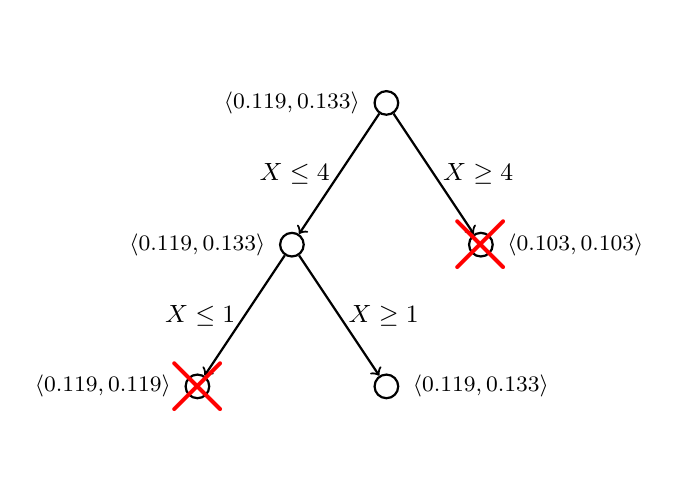
\begin{tikzpicture}
    [scale=.6,auto=left,every node/.style={draw, thick, circle, inner sep = 0pt, minimum width = 0.3cm}]
  \node (r) at (5,10) {};
  \node[draw=none, circle=none, minimum width=0.5cm, minimum height=0.2cm, inner sep=2pt] (l) at (3,10) {\footnotesize $\langle 0.119, 0.133 \rangle$};

  \node (l4) at (3,7) {};
  \node[draw=none, circle=none, minimum width=0.5cm, minimum height=0.2cm, inner sep=2pt] (l) at (1,7) {\footnotesize $\langle 0.119, 0.133 \rangle$};
  \node (g4) at (7,7) {};
  \node[draw=none, circle=none, minimum width=0.5cm, minimum height=0.2cm, inner sep=2pt] (l) at (9,7) {\footnotesize $\langle 0.103, 0.103 \rangle$};

  \node (l1) at (1,4) {};
  \node[draw=none, circle=none, minimum width=0.5cm, minimum height=0.2cm, inner sep=2pt] (l) at (-1,4) {\footnotesize $\langle 0.119, 0.119 \rangle$};
  \node (g1) at (5,4) {};
  \node[draw=none, circle=none, minimum width=0.5cm, minimum height=0.2cm, inner sep=2pt] (l) at (7,4) {\footnotesize $\langle 0.119, 0.133 \rangle$};

  \foreach \from/\to/\label/\pos in {r/l4/{$X \leq 4$}/left, r/g4/{$X \geq 4$}/right, l4/l1/{$X \leq 1$}/left, l4/g1/{$X \geq 1$}/right}
    \draw (\from) edge[->, thick] node[\pos, draw=none, circle=none, minimum width=0.5cm, minimum height=0.2cm, inner sep=2pt]{\small \label} (\to);

  \node[draw=none, color=red] at (7,7) {\scalebox{1.5}{\Huge $\times$}};
  \node[draw=none, color=red] at (1,4) {\scalebox{1.5}{\Huge $\times$}};
\end{tikzpicture}
\end{document}
